
% !TeX spellcheck = de_DE
\section{Geschäftsmodell}
\textbf{Definition:} A business model describes the rationale of how an organization \textit{creates}, \textit{delivers}, and \textit{captures} value. 

\subsection{Argumentationspfad}
\begin{multicols}{2}
	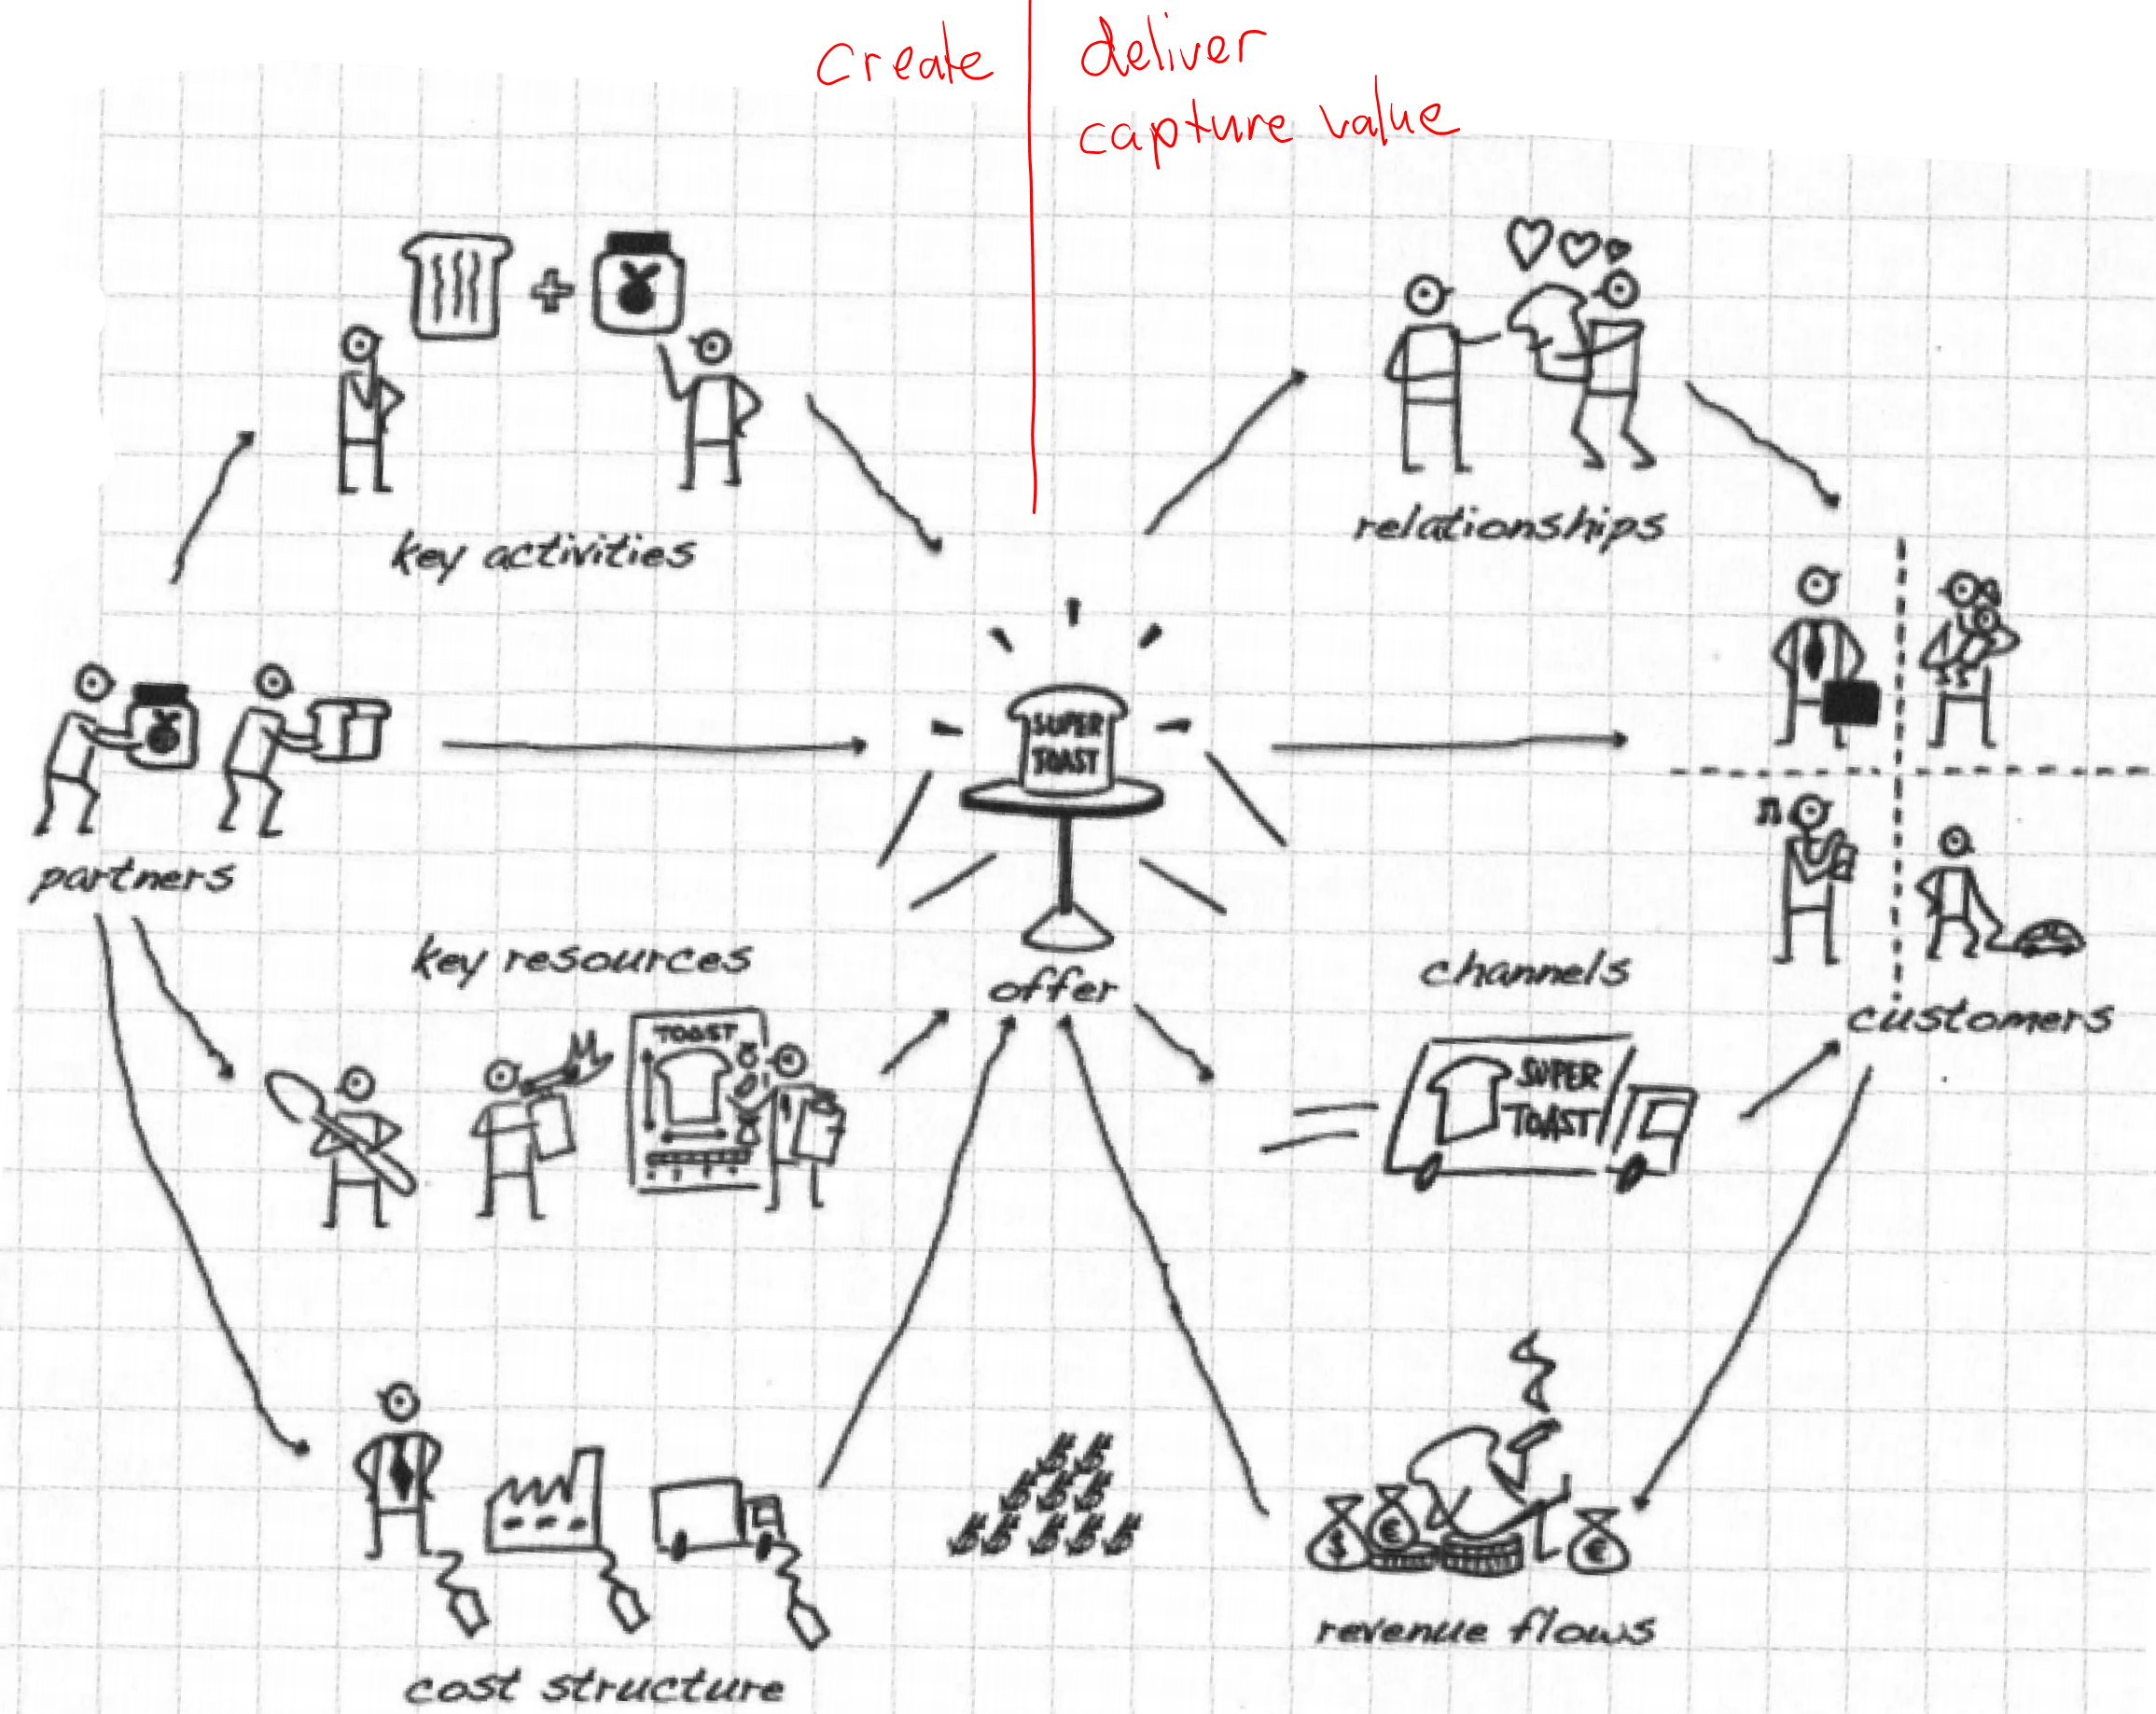
\includegraphics[width=1\linewidth]{images/Geschaeftsmodell}
	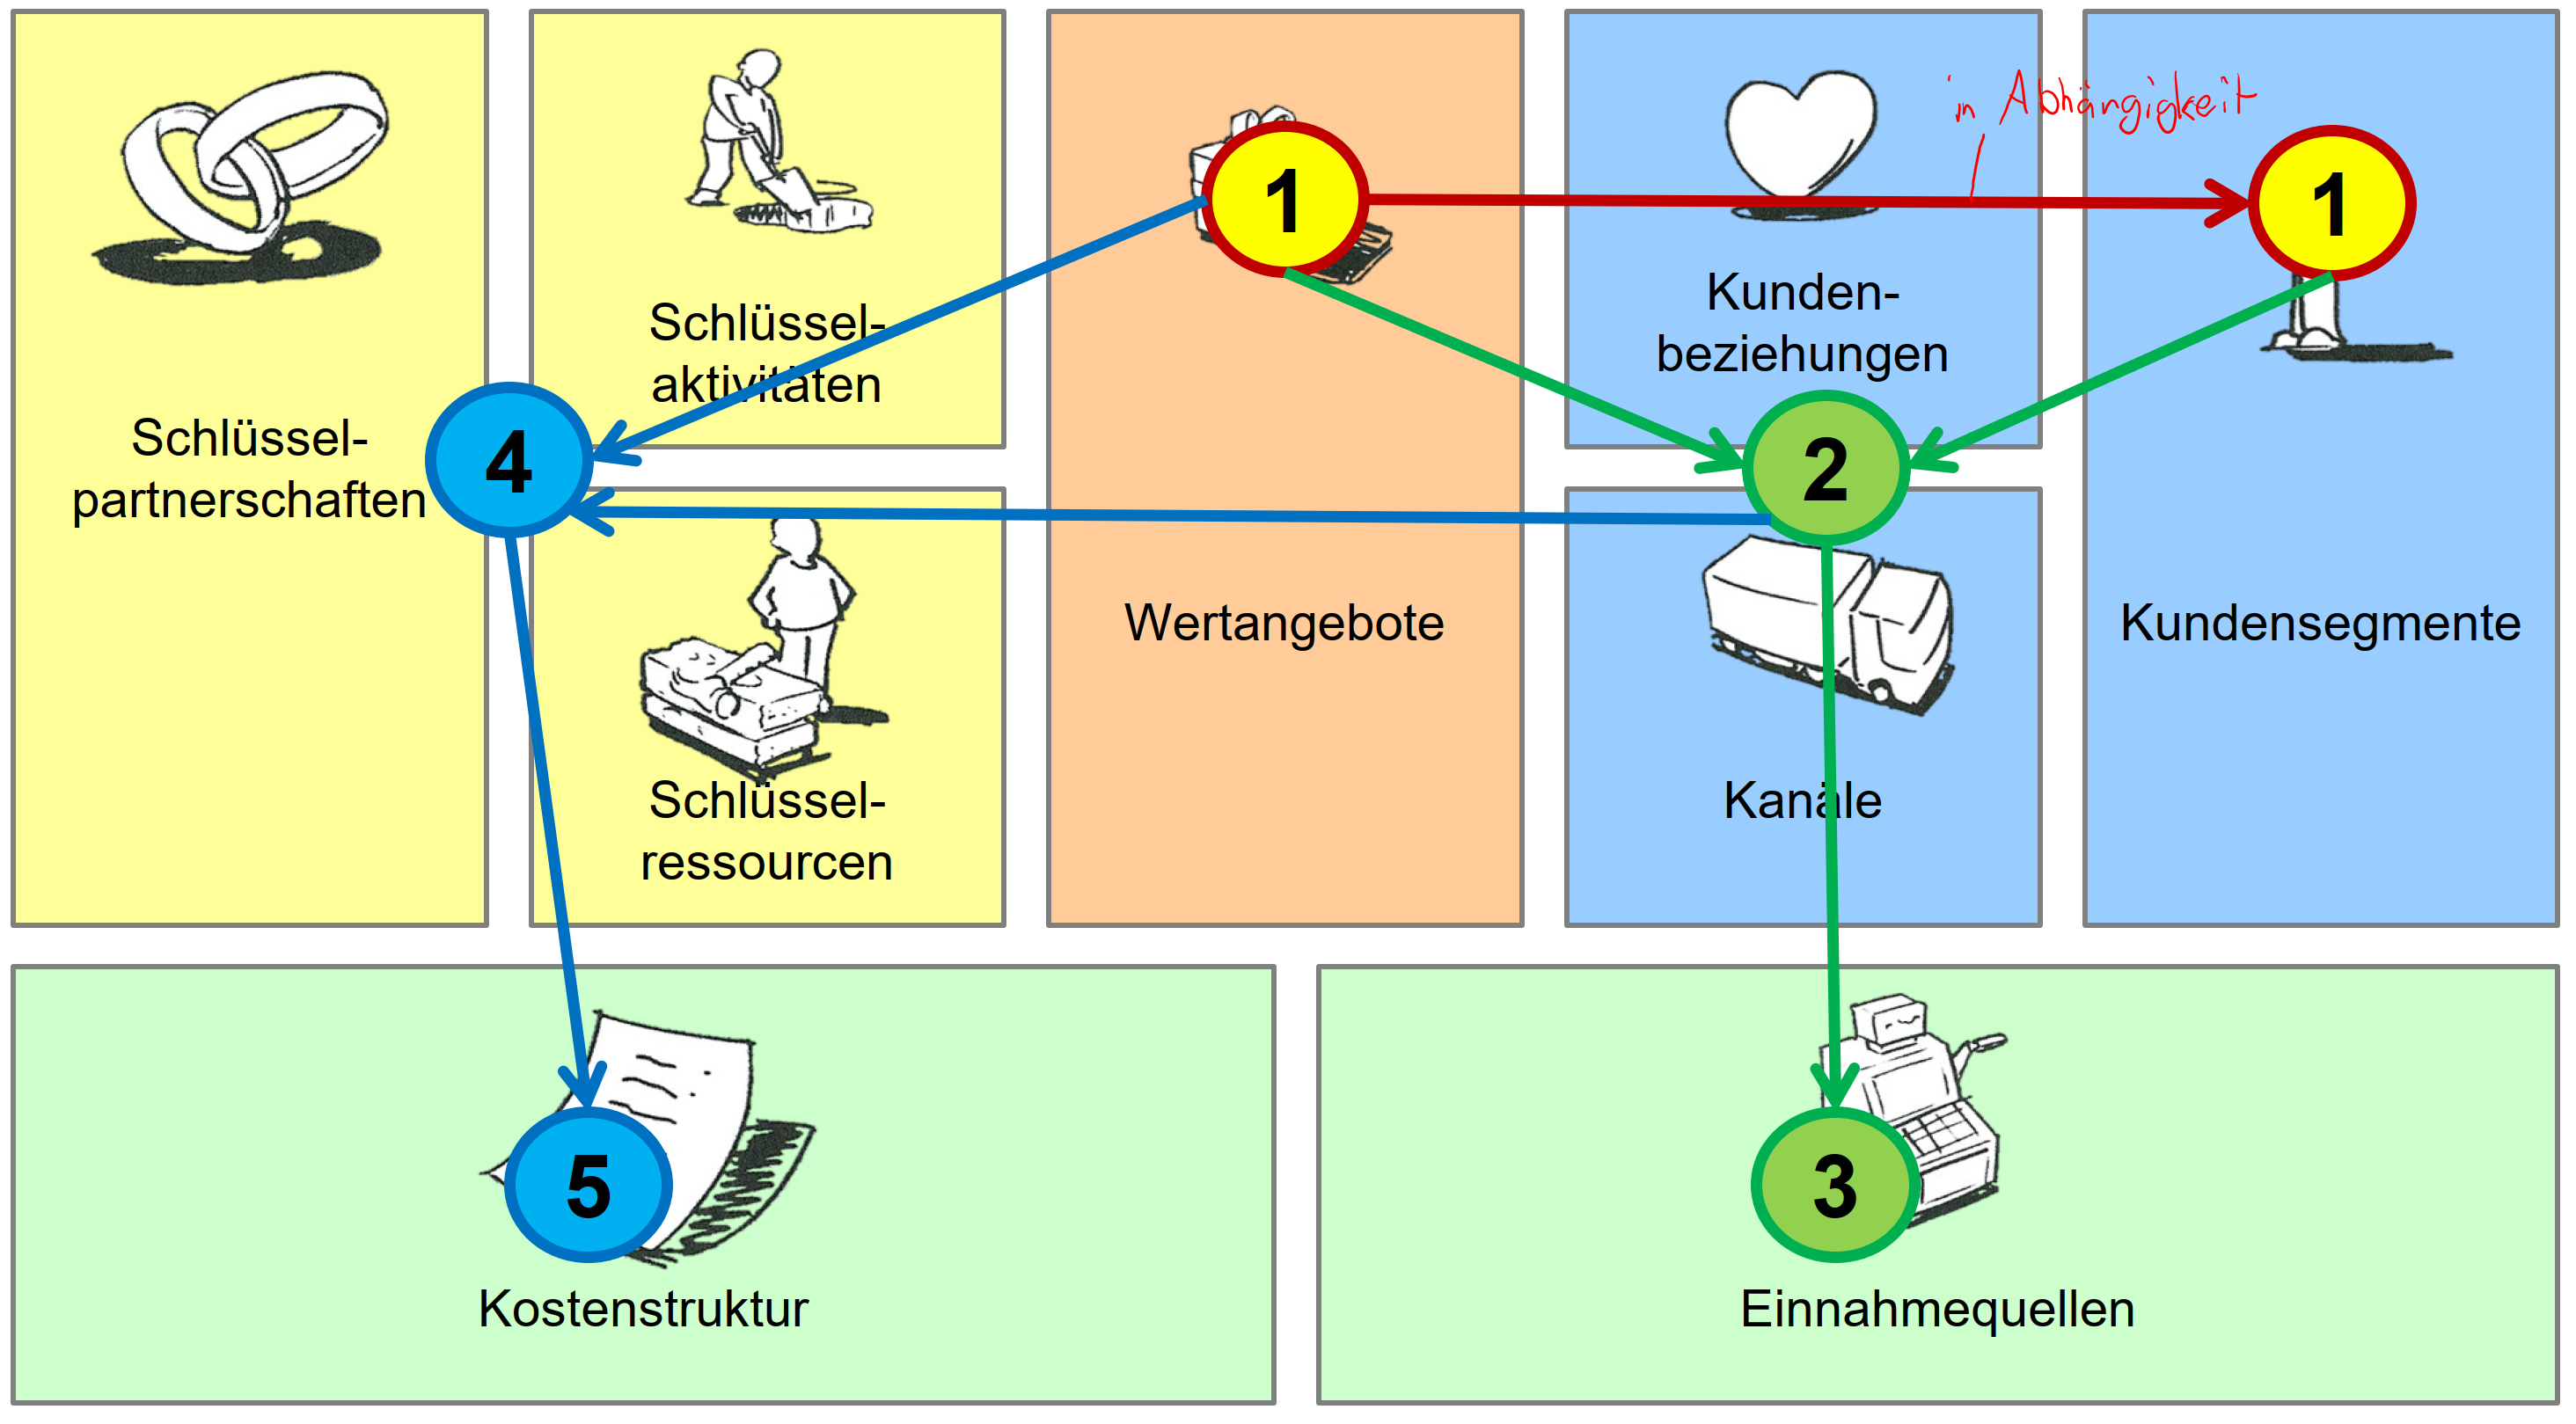
\includegraphics[width=1\linewidth]{images/Argumentationspfad}
\end{multicols}

\subsubsection{Wertangebot}
Paket von Produkten und Dienstleistungen, das für ein bestimmtes Kundensegment Wert schöpft.
\begin{itemize}
	\item Welchen Wert vermitteln wir dem Kunden?
	\item Welche der Probleme unseres Kunden helfen wir zu lösen?
	\item Welche Kundenbedürfnisse erfüllen wir?
	\item Welche Produkte und Dienstleistungspakete bieten wir jedem Kundensegment an?
\end{itemize}

\paragraph{Nutzen-Dimension}
An welcher Stelle bekommt der Nutzer etwas was er an anderer Stelle nicht bekommen würde? \\
\begin{multicols}{2}
	\begin{tabular}{|l|p{0.45\linewidth}|}
		\hline 
		\textbf{Nutzen-Dimension} & \textbf{Bemerkung, Beispiel}\\ \hline
		Neuheit & Neue Bedürfnisse, neue Technologien\\ \hline
		Leistung & Schneller, Präziser, Stärker, z.B. Fernseher\\ \hline
		Kundenwunsch & Massgeschneiderte Produkte\\ \hline
		Erleichterung & Rundumpaket, z.B. Rolls-Royce Triebwerke\\ \hline
		Design & Modebranche, Unterhaltungselektronik\\ \hline
		Marke / Status & Gutes Gefühl, persönliche Differenzierung z.B. Rolex\\ \hline
	\end{tabular} 

	\begin{tabular}{|l|p{0.45\linewidth}|}
		\hline 
		\textbf{Nutzen-Dimension} & \textbf{Bemerkung, Beispiel}\\ \hline		
		Preis & Investitionsgüter\\ \hline
		Kostenreduktion & Auslagerung von Aktivitäten, z.B. Cloud Computing\\ \hline
		Risikominderung & Garantieleistung, Versicherungen\\ \hline
		Verfügbarkeit & Sharing-Konzepte, z.B. Mobility oder Hapimag\\ \hline
		Bequemlichkeit & Einfachheit, Bedienbarkeit, z.B. Apple iPhone \\ \hline
	\end{tabular} 	
\end{multicols}

\paragraph{Produktebenen}
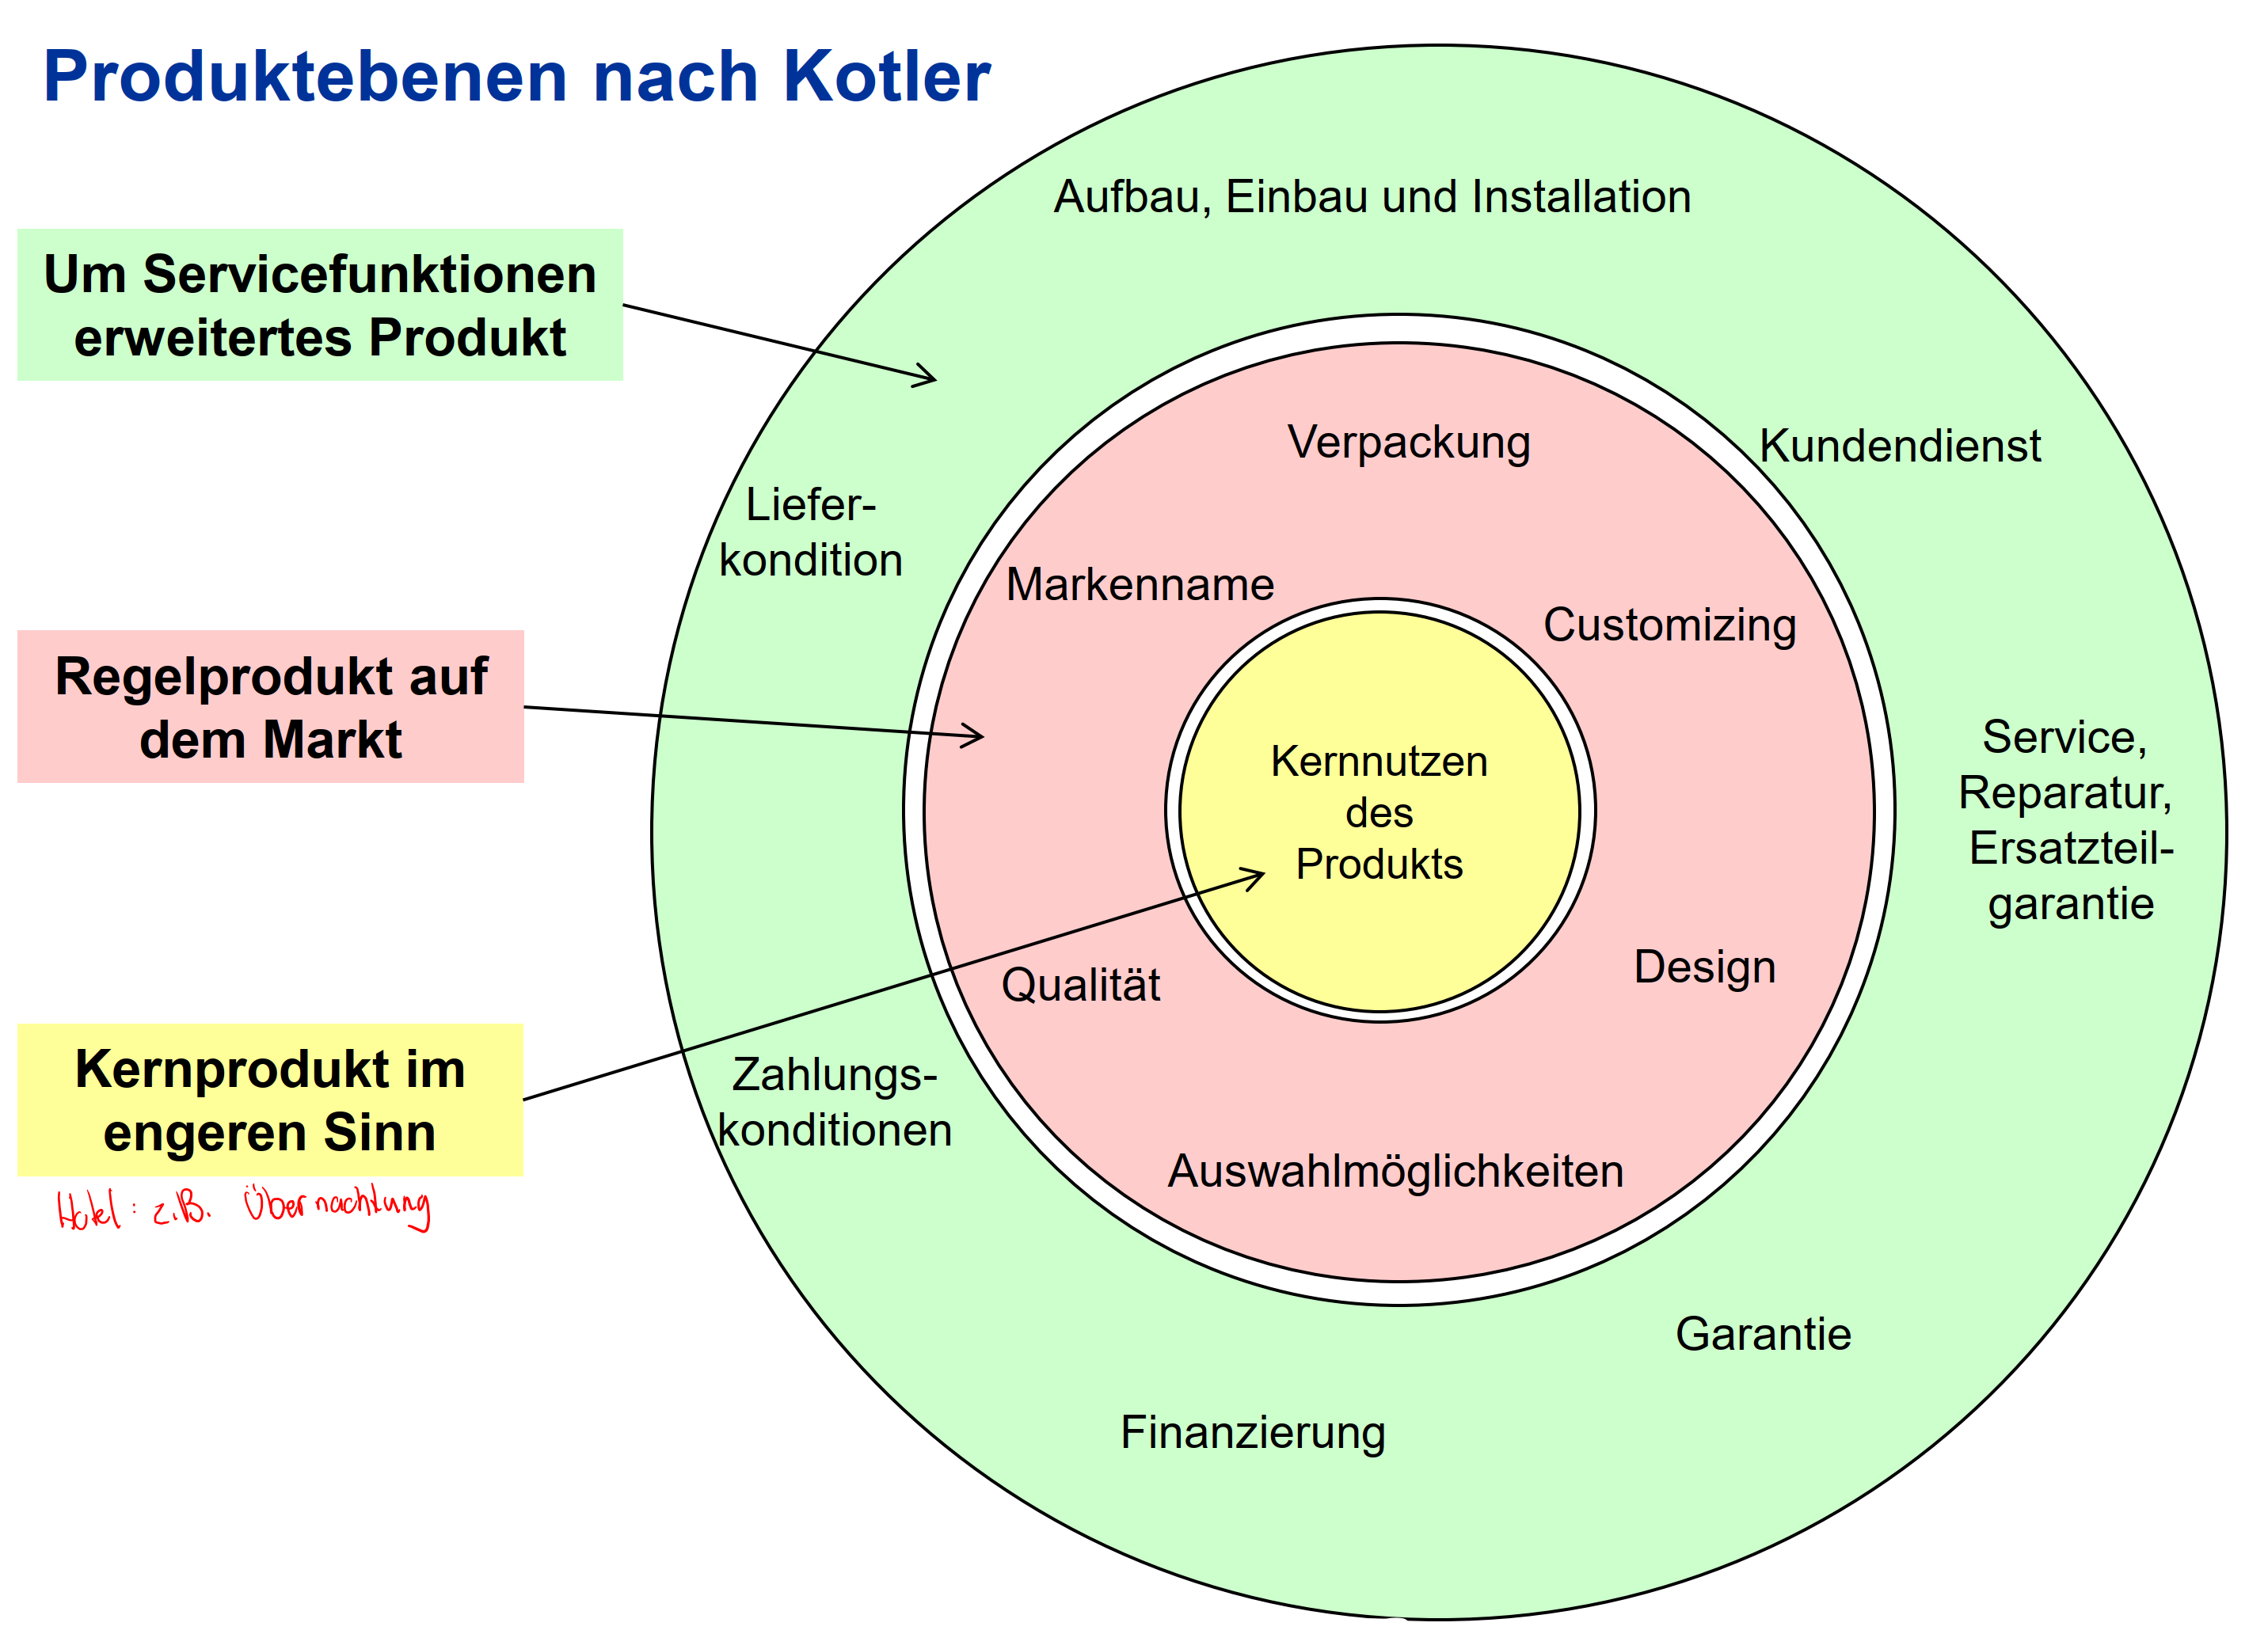
\includegraphics[width=0.5\linewidth]{images/Produktebenen}

\subsubsection{Kundensegmente}
Verschiedene Gruppen von Personen und Organisationen, die ein Unternehmen erreichen und bedienen will.
\begin{itemize}
	\item Für wen wird Wert generiert?
	\item Wer sind unsere wichtigsten Kunden?
\end{itemize}

\begin{tabular}{|p{0.1\linewidth}|p{0.85\linewidth}|}
	\hline 
	Bedürfnisse & Kunden haben die gleichen Bedürfnisse\\ \hline
	Kanäle & Kunden sind über gleiche Distributionskanäle erreichbar\\ \hline
	Beziehungen & Kunden erfordern gleiche Arten von Beziehungen\\ \hline
	Kaufkraft & Kunden weisen gleiche Zahlungsbereitschaft / Kaufkraft\\ \hline
	Messbarkeit & Segmente ist mit Marktforschungs-Methoden erfassbar\\ \hline
	Grösse & Grösse und Potenzial des Kundensegments erlauben profitable Bearbeitung\\ \hline
	Stabilität & Segment sollte mindestens für eine Planungsperiode stabil sein\\ \hline
\end{tabular} 

\subsubsection{Kanäle}
Beschreibt, wie ein Unternehmen seine Kundensegmente erreicht und anspricht, um ein Wertangebot zu vermitteln.
\begin{multicols}{2}	
	\begin{itemize}
		\item Über welche Kanäle wollen unsere Kunden erreicht werden?
		\item Wie erreichen wir sie jetzt?
		\item Wie sind unsere Kanäle integriert?
		\item Welche funktionieren am besten?
		\item Welche sind am kosteneffizientisten?
		\item Wie integrieren wir sie in die Kundenabläufe?
	\end{itemize}

	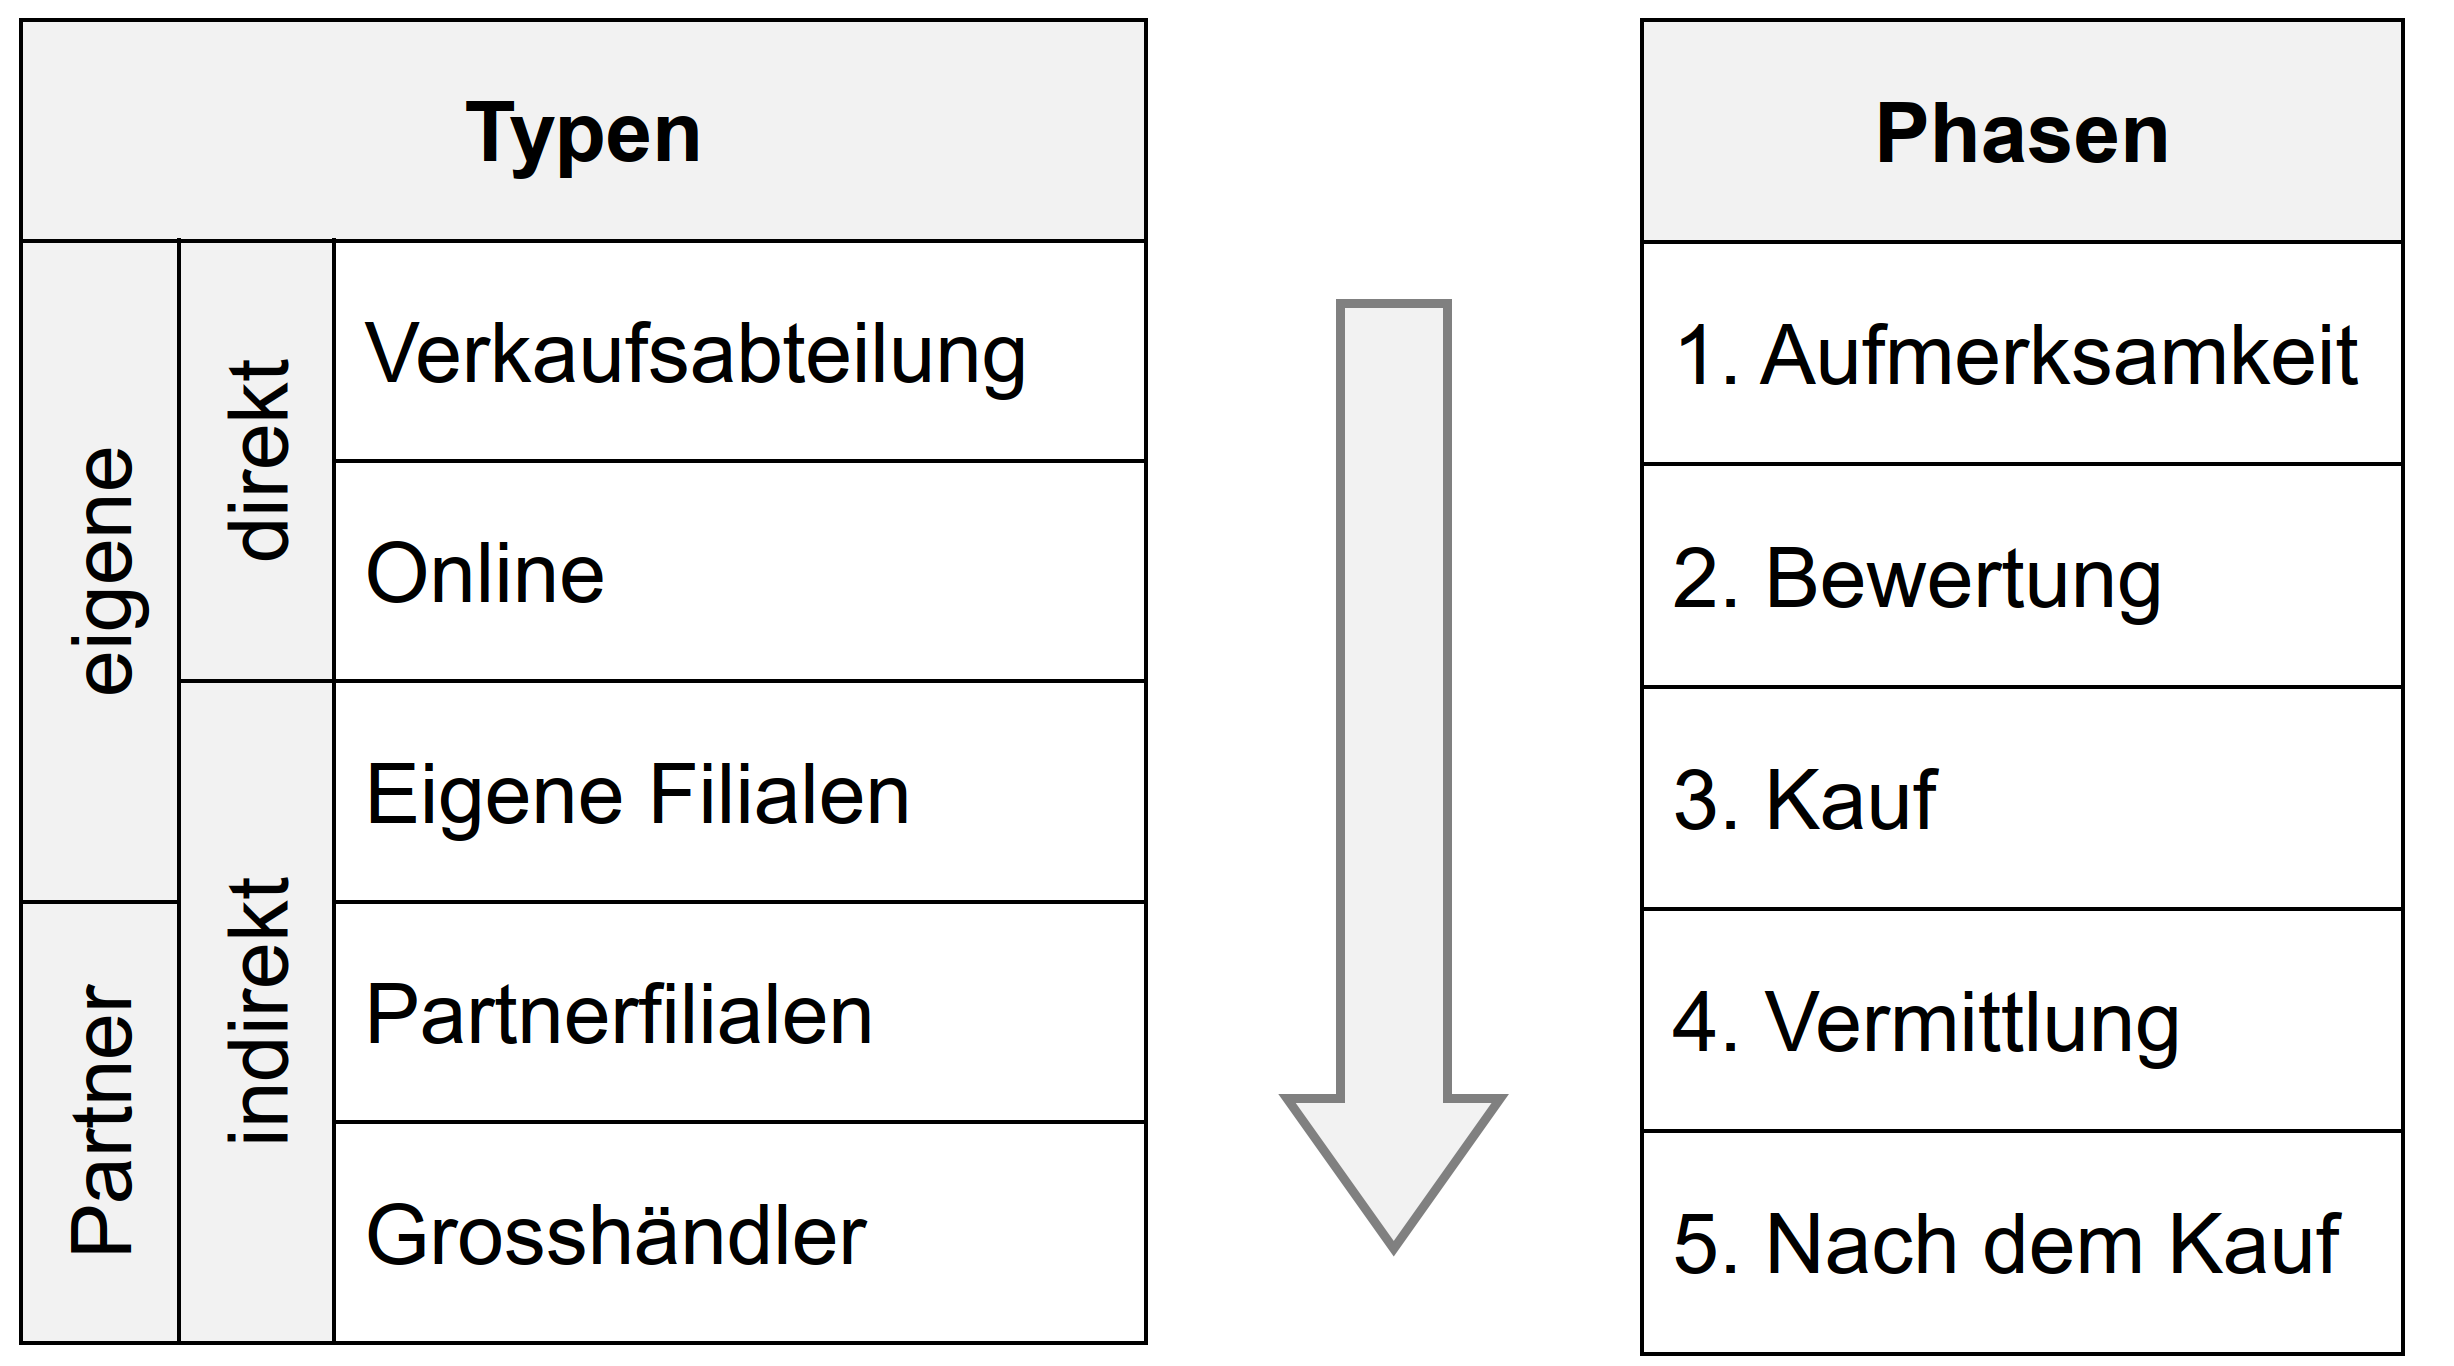
\includegraphics[width=1\linewidth]{images/Kanaele}
\end{multicols}

\subsubsection{Kundenbeziehungen}
Beschreibt die Arten von Beziehungen, die ein Unternehmen mit bestimmten Kundensegmenten eingeht.
\begin{itemize}
	\item Welche Art von Beziehungen erwartet jedes unserer	Kundensegmente von uns?
	\item Welche haben wir eingerichtet?
	\item Wie kostenintensiv sind sie?
	\item Wie sind sie in unser übriges Geschäftsmodell integriert?
	\item Wie intensiv, persönlich/unpersönlich soll es sein?
\end{itemize}

\paragraph{Kategorien}
\begin{multicols}{3}
	\begin{itemize}
		\item Persönliche Unterstützung 
		\item Individuelle persönliche 	Unterstützung 
		\item Selbstbedienung 
		\item Kundensegment
		\item Automatisierte Dienstleistungen 
		\item Communities
		\item Mitbeteiligung
	\end{itemize}
\end{multicols}

\subsubsection{Einnahmequellen}
Einkünfte, die ein Unternehmen aus jedem Kundensegment bezieht.
\begin{itemize}
	\item Für welche Werte sind unsere Kunden wirklich zu bezahlen bereit?
	\item Wofür bezahlen sie jetzt?
	\item Wie bezahlen sie jetzt?
	\item Wie würden sie gerne bezahlen?
	\item Wie viel trägt jede Einnahmequelle zum Gesamtumsatz bei?
\end{itemize}

\paragraph{Kategorien}
\begin{multicols}{3}
	\begin{itemize}
		\item Verkauf von Produkten/Dienstleistungen 
		\item Nutzungsabhängige Gebühr 
		\item Mitgliedschaftsgebühr/Abonnement 
		\item Verleih/Vermietung/Leasing
		\item Lizenzen
		\item Maklergebühren
		\item Werbung
	\end{itemize}
\end{multicols}

\subsubsection{Schlüsselressourcen}
Beschreibt die wichtigsten Wirtschaftsgüter, die für das Funktionieren eines Geschäftsmodells notwendig sind.
\begin{itemize}
	\item Welche Schlüsselressourcen erfordern unsere Wertangebote?
	\item Unsere Distributionskanäle?
	\item Unsere Kundenbeziehungen?
	\item Unsere Einnahmequellen?
\end{itemize}

\paragraph{Kategorien}
\begin{multicols}{4}
	\begin{itemize}
		\item Physisch
		\item Intellektuell
		\item Menschlich
		\item Finanziell
	\end{itemize}
\end{multicols}

\subsubsection{Schlüsselaktivitäten}
Beschreibt die wichtigsten Dinge, die ein Unternehmen tun muss, damit sein Geschäftsmodell funktioniert.
\begin{itemize}
	\item Welche Schlüsselaktivitäten erfordern unsere Wertangebote?
	\item Unsere Distributionskanäle?
	\item Unsere Kundenbeziehungen?
	\item Unsere Einnahmequellen?
\end{itemize}

\paragraph{Kategorien}
\begin{multicols}{3}
	\begin{itemize}
		\item Produktion
		\item Problemlösung
		\item Plattform und Netzwerk
	\end{itemize}
\end{multicols}

\subsubsection{Schlüsselapartnerschaften}
Netzwerk von Lieferanten und Partnern, die zum Gelingen des Geschäftsmodells beitragen.
\begin{itemize}
	\item Wer sind unsere Schlüsselpartner?
	\item Wer sind unsere Schlüssellieferanten?
	\item Welche Schlüsselressourcen beziehen wir von Partnern?
	\item Welche Schlüsselaktivitäten üben Partner aus?
\end{itemize}

\subsubsection{Kostenstruktur}
Alle Kosten, die bei der Ausführung des Geschäftsmodells anfallen.
\begin{itemize}
	\item Welches sind die wichtigsten mit unserem Geschäftsmodell verbundenen Kosten?
	\item Welche Schlüsselressourcen sind am teuersten?
	\item Welche Schlüsselaktivitäten sind am teuersten?
\end{itemize}

\paragraph{Wichtigste Grössen}
\begin{itemize}
	\item \textbf{Fixkosten:} Kosten, die unabhängig von der produzierten Menge gleich bleiben wie Löhne und Mieten
	\item \textbf{Variable Kosten:} Kosten die sich mit der produzierten Menge verändern, wie Material- und	Energiekosten.
	\item \textbf{Deckungsbeitrag (DB):} Der DB stellt die tatsächlichen Umsatzerlöse den direkten Kosten für die Erstellung eines verkauften Produktes / Bereiches gegenüber. (Deckungsbeitrag = Verkaufspreis pro Stück - Direkte Kosten pro Stück)
\end{itemize}

\begin{tabular}{|p{0.15\linewidth}|p{0.8\linewidth}|}
	\hline 
	Sachkosten & Anschaffungskosten für Maschinen, Geräte, Produktionswerkzeuge	Technologie \& Aufwendungen zur Bereitstellung und zum Betrieb der Informationstechnologie.\\ \hline
	Materialkosten & Benötigte Rohstoffe oder Materialien zur Erstellung eines Produktes oder zur Umsetzung eines Vorhabens.\\ \hline
	Personalkosten & Alle Aufwendungen zur Bereitstellung von Personaldiensten.\\ \hline
	Marketing und Vertrieb & Alle Aufwendungen, die für geplante Marketing- und Vertriebsaktivitäten anfallen.\\ \hline
	Administration & Aufwendungen für Miete, Leasinggebühren oder ähnliche Kosten, welche dem erstellen Produkt direkt oder als Gemeinkosten anteilmässig zugeordnet werden.\\ \hline
	Logistik & Kosten, die bei der Verteilung oder Auslieferung des Produktes anfallen.\\ \hline
	Support & Aufbau und Betrieb von Supportfunktionen (Kundensupport) sowie Instandhaltungs- und Reparaturkosten von Maschinen und Geräten.\\ \hline
	Schutzrecht & Für Innovationen fallen Kosten an für Patente, Lizenzen oder Designs.\\ \hline
\end{tabular} 